\chapter{视觉中的数学问题}

\section{最大似然估计}

\section{边缘化}	


\section{流形上的优化}
位置、速度定义在欧式空间,可以直接进行优化处理。在欧式空间定义,特性是对加法操作封闭,比如$\textbf{t}_2=\textbf{t}_1+\bigtriangleup \textbf{t}$。但是姿态,只对乘法操作封闭$\textbf{R}_2=\bigtriangleup \textbf{R}*\textbf{R}_1$,需要在流形空间中进行优化。\\
简单说,流形是一个非线性空间,但是在局部空间内对其进行线性化,就可以用线性空间进行拟合。
\indent 对于一般的优化问题:
\begin{equation}
x=
\end{equation}


在流形上优化的好处:\\
1、有约束优化问题转化为无约束优化问题,如det(R)=1,有约束的优化问题会引入拉格朗日因子,优化变量维数会更高, 转换 李代数后,没有什么约束了,


\section{Lie algebra扰动}

对于$\xi\in se(3)$定义\\
\begin{align}
	\xi^\wedge &=
	\left[ \begin{array}{c}   %该矩阵一共3列,每一列都居中放置
	\rho \\  %第一行元素
	\phi \\  %第二行元素
	\end{array}	\right] = 
	\left[ \begin{array}{cc}
	   \phi^\wedge \quad  \rho \\
	    0^T        \quad  0
	\end{array} \right] \in R^{4x4},\rho,\phi\in R^3 \\	
	\xi^\wedge &=1
	\left[ \begin{array}{c}   %该矩阵一共3列,每一列都居中放置
      	\rho \\  %第一行元素
    	\phi \\  %第二行元素
	\end{array}	\right] = 
	\left[ \begin{array}{cc}
    	\phi^\wedge \quad  \rho^\wedge \\
    	0^T         \quad  \phi^\wedge
	\end{array} \right] \in R^{4x4},\rho,\phi\in R^3
\end{align}


\section{SE(3)伴随矩阵}




\section{矩阵正交化}
矩阵正交化本是矩阵问题,放在几何部分中,是因为想从几何的角度中来阐述。\\
本小节内容参见:https://blog.csdn.net/tengweitw/article/details/41174555、\\
https://blog.csdn.net/tengweitw/article/details/41775545\\

\subsection*{矩阵正交投影}

\begin{figure}[h]%%图
	\centering  %插入的图片居中表示
	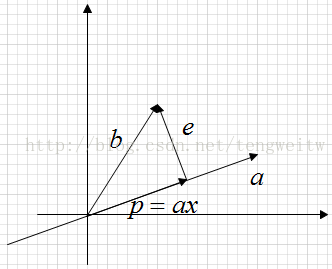
\includegraphics[width=0.7\linewidth]{math/img/1}  %插入的图,包括JPG,PNG,PDF,EPS等,放在源文件目录下
	\caption{向量b在向量a上的投影.}  %图片的名称
	\label{fig:mcmthesis-logo}   %标签,用作引用
\end{figure}
\noindent 图中,$\textit{\textbf{e}}=\textit{\textbf{b}}-\textit{\textbf{p}}=\textit{\textbf{b}}-x\textit{\textbf{a}}$,向量\textit{\textbf{e}}为投影残差\\
向量\textit{\textbf{a}}与向量\textit{\textbf{e}}垂直,\\ 
$\textit{\textbf{a}}^T\textit{\textbf{e}}=0 \longrightarrow \textit{\textbf{a}}^T(\textit{\textbf{b}}-x\textit{\textbf{a}})=0 \longrightarrow x\textit{\textbf{a}}^T\textit{\textbf{a}}=\textit{\textbf{a}}^T\textit{\textbf{b}} \longrightarrow x = \frac{\textbf{\textit{a}}^T\textbf{\textit{b}}}{\textbf{\textit{a}}^T\textbf{\textit{a}}}$\\
$x$是一个标量值,刻画了向量b投影到向量a上的长度。\\
\begin{center}
$\textbf{\textit{p}}=\textbf{\textit{a}}x = \textbf{\textit{a}}\frac{\textbf{\textit{a}}^T\textbf{\textit{b}}}{\textbf{\textit{a}}^T\textit{\textbf{a}}}$\\
\end{center}
\textbf{P}为投影矩阵,$\textbf{P}\textit{\textbf{b}}=\textit{\textbf{p}}$,则:
\begin{center}
$\textbf{P}=\frac{\textit{\textbf{a}}\textit{\textbf{a}}^T}{\textit{\textbf{a}}^T\textit{\textbf{a}}}$	
\end{center}


\subsection*{Gram-Schmidt正交化}
